\documentclass[a4paper,11pt]{article}

\usepackage{mlsubmit, graphicx, subcaption}

\begin{document}

\initmlsubmision{3} % assignment number
{Piyush Bagad}   % your name
{150487}	% your roll number

\begin{mlsolution}

The soft-margin linear SVM dual objective to compute weights can be stated as
\[
\arg\max_{0 \leq \alpha\leq C} f(\vec{\alpha})
\]
where $ f(\vec{\alpha}) = \vec{\alpha}^{T}.\vec{1} - \frac{1}{2}\vec{\alpha}^{T}\vec{G}\vec{\alpha}  $. The gradient-ascent step that we consider for $\alpha_n$ is:
\[
\alpha_n = \alpha_n + \delta_{*}; \ \ \text{where } \  \delta_{*} := \arg\max_{\delta} f(\vec{\alpha}+\delta\vec{e}_{n})
\]
First, we will have to compute $\delta_{*}$ in order to apply the ascent step.
\[
f(\vec{\alpha}+\delta\vec{e}_n) = (\vec{\alpha}+\delta\vec{e}_{n})^{T}.\vec{1} - \frac{1}{2}(\vec{\alpha}+\delta\vec{e}_{n})^{T}\vec{G}(\vec{\alpha}+\delta\vec{e}_{n})
\]
\[
\therefore 
f(\vec{\alpha}+\delta\vec{e}_n) = \vec{\alpha}^{T}.\vec{1} +\delta\vec{e}^{T}_{n}.\vec{1} - \frac{1}{2}\vec{\alpha}^{T}\vec{G}\alpha     - \frac{1}{2}\vec{\alpha}^{T}\vec{G}\delta\vec{e}_{n} - \frac{1}{2}\delta\vec{e}^{T}_{n}\vec{G}\alpha - \frac{1}{2}\delta\vec{e}^{T}_{n}\vec{G}\delta \vec{e}_{n}
\]
\[
f(\vec{\alpha}+\delta\vec{e}_n) = f(\alpha) +\delta(\vec{e}^{T}_{n}.\vec{1} - \vec{\alpha}^{T}\vec{G}\vec{e}_{n}) - \frac{1}{2}\delta^{2}\vec{e}^{T}_{n}\vec{G} \vec{e}_{n}
\]
Taking partial derivative w.r.t. $\delta$, and equating it to 0, we get
\[
\frac{\partial f(\vec{\alpha}+\delta\vec{e}_n)}{\partial\delta} = (\vec{e}^{T}_{n}.\vec{1} - \vec{\alpha}^{T}\vec{G}\vec{e}_{n}) - \delta\vec{e}^{T}_{n}\vec{G}\vec{e}_{n}
\]
\begin{equation}
\label{delta}
\Rightarrow \boxed{\delta_{*} = \frac{\vec{e}^{T}_{n}.\vec{1} - \vec{\alpha}^{T}\vec{G}\vec{e}_{n}}{\vec{e}^{T}_{n}\vec{G}\vec{e}_{n}}}
\end{equation}
Note that we want to ensure that $0 \leq \alpha^{(t)}_n\leq C$, thus if the update value for $\alpha_n$ becomes $\geq C$, we will just set it to $C$ and if it goes less $0$, we will just set it to $0$. Thus, the update for $\alpha_n$ will become as follows:
\begin{equation}
\label{alpha}
\alpha^{(t)}_n =
\begin{cases}
0, & \text{if } \alpha^{(t-1)}_n+\delta_{*} < 0\\
C, & \text{if } \alpha^{(t-1)}_n+\delta_{*} > C\\
\alpha^{(t-1)}_n+\delta_{*} & \text{otherwise}
\end{cases} 
\end{equation}


\subsection{Coordinate ascent algorithm sketch}
\begin{enumerate}
	\item Inititalize $\alpha = \alpha^{(0)} = [\alpha^{(0)}_{1}, .., \alpha^{(0)}_{N}]$
	\item Randomly choose $n \in \{1,2,..,N\}$. Compute $\delta_{*}$ from equation \ref{delta}. 
	\item Update $\alpha^{(t)}_n$ in terms of $\alpha^{(t-1)}_{n}$ and $\delta_{*}$ as in equation \ref{alpha}.
	\item If not converged, go to step 2.
\end{enumerate}

\end{mlsolution}

\begin{mlsolution} 
Let $\hat{f}$ be the function learnt by minimizing $\mathcal{L}_{W}$ , which is defined as the sum of squared distances between all pairs of points that are within the same cluster, i.e.,
\[
\hat{f} = \arg \min_{f} \sum_{n,m} \mathbb{I}(f_n = f_m)\Vert\vec{x}_{n} - \vec{x}_{m}\Vert^{2}
\]
Note that we can write the indicator function as follows:
\[
\mathbb{I}(f_n = f_m) = 1 - \mathbb{I}(f_n \neq f_m)
\]
Thus, replacing in the loss function, we obtain
\[
\hat{f} = \arg \min_{f} \left[ \sum_{n,m} \Vert\vec{x}_{n} - \vec{x}_{m}\Vert^{2} - \sum_{n,m}\mathbb{I}(f_n \neq f_m) \Vert\vec{x}_{n} - \vec{x}_{m}\Vert^{2} \right] 
\]
We can re-write it as follows, since the first term does not involve the argument for minimization. Essentially, it remains to be a constant w.r.t the minimization.
\[
\therefore \hat{f} = \sum_{n,m} \Vert\vec{x}_{n} - \vec{x}_{m}\Vert^{2} - \arg \min_{f}  \sum_{n,m}\mathbb{I}(f_n \neq f_m) \Vert\vec{x}_{n} - \vec{x}_{m}\Vert^{2}  
\]
\[
\therefore \hat{f} = - \arg \min_{f}  \sum_{n,m}\mathbb{I}(f_n \neq f_m) \Vert\vec{x}_{n} - \vec{x}_{m}\Vert^{2}
\]
\[
\boxed{\therefore \hat{f} = \arg \max_{f}  \sum_{n,m}\mathbb{I}(f_n \neq f_m) \Vert\vec{x}_{n} - \vec{x}_{m}\Vert^{2}}
\]
Hence, it turns out to be equivalent to maximizing the inter-cluster distances - distance between points of different clusters. 
\end{mlsolution}

\begin{mlsolution}
Let $X=\{\textbf{x}_1, \textbf{x}_2,..,\textbf{x}_N\}, \ \Theta=\{\mu, \Sigma\}$ and 
\[
p(x_n| \Theta) = \mathcal{N}(x_n| \Theta)
\]


\subsection{Part 1: Estimating the conditional given current parameter estimates}
\label{p3p1}
Let's say we have $\Theta$ as our current parameter estimates. Let us try to estimate the missing part of data for point $x_n$. We have
\[
p([x^{obs}_n, x^{miss}_n]| \Theta) = \mathcal{N}([x^{obs}_n, x^{miss}_n]| \Theta)
\]
Based on the missing and observed part of this data point, let us denote the paramters as follows:
\[
\mu = \begin{pmatrix}
\mu_{miss} \\ 
\mu_{obs} 
\end{pmatrix}
 = \begin{pmatrix}
 \mu_{1} \\ 
 \mu_{2} 
 \end{pmatrix}, \ 
\Sigma = \begin{pmatrix}
\Sigma_{11} & \Sigma_{12}\\
\Sigma_{21} & \Sigma_{22}\\
\end{pmatrix}
\]
Note that this miss-observed split may be different for different examples. This also makes intuitive sense, for example, if for the first example the first two features are missing, then its estimate should be based on the means of these features of other examples and also covariances with other features. For an example with different set of missing features, the estimates will be different.
Since a conditional of  a gaussian is a gaussian, using result theorem 4.3.1 from MLAPP, we have
\[
\boxed{p(x^{miss}_{n}| x^{obs}_{n}, \Theta) = \mathcal{N}(x^{miss}_n| x^{obs}_{n}, \{\mu_{miss|obs}, \Sigma_{miss|obs}\})} \ \text{where}
\]
\[
\mu_{miss|obs} = \mu_{1} + \Sigma_{12}\Sigma^{-1}_{22}(\textbf{x}^{obs}_n-\mu_{2})
\]
\[
\Sigma_{miss|obs} = \Sigma_{11}-\Sigma_{12}\Sigma^{-1}_{22}\Sigma_{21}
\]

\subsection{Part 2: Expected CLL}
First, I will compute the $CLL$ as follows and then take the expectation:
\[
CLL = \sum_{n=1}^{N}\log p(\textbf{x}_n| \Theta=\{\mu, \Sigma\}) 
\]
\[
CLL = \sum_{n=1}^{N}\log p([\textbf{x}^{obs}_n, \textbf{x}^{miss}_n]| \Theta=\{\mu, \Sigma\})
\]
\[
\mathbb{E}[CLL] = \sum_{n=1}^{N}\mathbb{E}\left[ \log p([\textbf{x}^{obs}_n, \textbf{x}^{miss}_n]| \mu, \Sigma) \right] 
\]
\[
\boxed{\mathbb{E}[CLL] = \text{constant} \ + \frac{N}{2}(log |\Sigma|^{-1}) - \frac{1}{2}\text{Trace}(\Sigma^{-1}\mathbb{E}[S])}
\]
\[
S = \sum_{n=1}^{N} (\textbf{x}_{n}-\mu)(\textbf{x}_{n}-\mu)^{T}
\]
We will need to compute the expectation of $S$ over the posterior. Note that, we will have the following expectation values:
\begin{equation}
\label{eq1}
\mathbb{E}[\textbf{x}_n] = \begin{pmatrix}
\mathbb{E}[\textbf{x}^{obs}_n] \\
\mathbb{E}[\textbf{x}^{miss}_n] 
\end{pmatrix} = \begin{pmatrix}
\textbf{x}^{obs}_n \\ 
\mathbb{E}[\textbf{x}^{miss}_n] 
\end{pmatrix}
\end{equation}
\begin{equation}
\label{eq2}
\mathbb{E}[\textbf{x}_{n}\textbf{x}^{T}_{n}] = \begin{pmatrix}
\textbf{x}^{obs}_{n}\textbf{x}^{(obs)T}_{n} & \textbf{x}^{obs}_{n}\mathbb{E}[\textbf{x}^{miss}_{n}]^{T} \\
\mathbb{E}[\textbf{x}^{miss}_{n}](\textbf{x}^{obs}_{n})^{T} & \mathbb{E}[\textbf{x}^{miss}_{n}(\textbf{x}^{miss}_{n})^{T}]
\end{pmatrix}
\end{equation}
\begin{equation}
\label{eq3}
\mathbb{E}[S] = \sum_{n=1}^{N}\left\lbrace \mathbb{E}[\textbf{x}_{n}\textbf{x}^{T}_{n}] + \mu \mu^{T} - 2\mu \mathbb{E}[\textbf{x}_n]^{T} \right\rbrace
\end{equation}
Note that from part \ref{p3p1}, we have got the conditional distribution for $\textbf{x}^{miss}_{n}$, thus we will have the mean $\mathbb{E}[\textbf{x}^{miss}_{n}] = \mu_{miss|obs}$. The expected CLL computation is over the conditional distribution. Thus, we can plug the value of $\mathbb{E}[\textbf{x}^{miss}_{n}]$ in the above equations to obtain the expected CLL. The only computation that will remain is 
\[
\mathbb{E}[\textbf{x}^{miss}_{n}(\textbf{x}^{miss}_{n})^{T}] = \mathbb{E}[\textbf{x}^{miss}_{n}]\mathbb{E}[\textbf{x}^{miss}_{n}]^{T} + cov(\textbf{x}^{miss}_{n}) =  \mathbb{E}[\textbf{x}^{miss}_{n}]\mathbb{E}[\textbf{x}^{miss}_{n}]^{T} + \Sigma_{11}
\]

\subsection{Part 3: Estimation of parameters: M step}
Let us denote $\mathbb{E}[CLL] = \mathcal{L}(\mu, \Sigma)$. In order to obtain the updates for these paramteres, we will set the partial derivatives to 0 treating terms involving $\mathbb{E}[\textbf{x}^{miss}_n]$ as constant. 
\[
\frac{\partial \mathcal{L}}{\partial \mu} = -\frac{1}{2}(\Sigma^{-1})^{T}\frac{\partial \mathbb{E}[S]}{\partial \mu}
\]
\[
\frac{\partial \mathbb{E}[S]}{\partial \mu} = \sum_{n=1}^{N} \left\lbrace \frac{\partial \mu\mu^{T}}{\partial \mu} -2\frac{\partial (\mu \mathbb{E}[\textbf{x}_n]^{T})}{\partial \mu}\right\rbrace 
\]
\[
\frac{\partial \mathbb{E}[S]}{\partial \mu} = N\frac{\partial \mu\mu^{T}}{\partial \mu}  - 2\sum_{n=1}^{N}\frac{\partial ([\mu \textbf{x}_{n}^{obs(T)}  \ \ \mu \mathbb{E}[\textbf{x}_{n}^{miss}]^{T}])}{\partial \mu}
\]
\[
\frac{\partial \mathcal{L}}{\partial \Sigma} = \frac{N|\Sigma|}{2}\frac{\partial |\Sigma|^{-1}}{\partial \Sigma} - \frac{1}{2} \frac{\partial \text{Trace}(\Sigma^{-1}\mathbb{E}[S])}{\partial \Sigma}
\]

\subsection{EM Algorithm steps:}
\begin{enumerate}
	\item Initialize $\Theta = \Theta^{(0)} = \{\mu^{(0)}, \Sigma^{(0)}\}$, set $t = 1$
	\item \textbf{E step}: Now, assuming the values of $\Theta^{(t-1)}$, compute the expected CLL using expression for $\mathbb{E}[S]$ (\ref{eq3}) which in turn needs the equations \ref{eq1} and \ref{eq2}.
	\item \textbf{M step}: Now, update the values for $\mu^{(t)}$ and $\Sigma^{(t)}$ using the equations ----. Update $t = t+1$.
	\item Repeat steps 2-4 until convergence.
\end{enumerate}

\end{mlsolution}

\begin{mlsolution}
Let us fix the following notation: $X_1 = \{(\textbf{x}_n, y_n)\}^{N}_{n=1}$, $X_2 = \{x_m\}^{N+M}_{m=N+1}$ and let $Z_2 = \{z_m\}^{N+M}_{m=N+1}$ be the latent variables. The set of parameters is $\Theta = \{\mu_k,\Sigma_{k}, \pi_{k} \}^{K}_{k=1}$. We assume that all the examples, whether with known labels or not are i.i.d sampled. We have the conditional distribution as follows:
\begin{eqnarray}
p(z_m = k| x_m, X_1, \Theta) = p(z_m = k| x_m, \Theta)  \\ =  \frac{p(x_m|z_m = k, \Theta)p(z_m = k|\Theta)}{p(x_m| \Theta)} \\ = \frac{p(x_m|z_m = k, \Theta)p(z_m|\Theta)}{\sum_{l=1}^{K}p(x_m, z_m = l|\Theta)}
\end{eqnarray}
\[
\text{Let } \gamma_{mk} = p(z_m = k| x_m, X_1, \Theta) = \frac{\pi_{k}\mathcal{N}(x_m| \mu_k, \Sigma_k)}{\sum_{l=1}^{K}\pi_{l}\mathcal{N}(x_m| \mu_l, \Sigma_l)}
\]
\begin{equation}
\label{eq4}
\boxed{\gamma_{mk}  = \frac{\pi_{k}\mathcal{N}(x_m| \mu_k, \Sigma_k)}{\mathcal{N}\left( \sum_{l}\pi_{l}\mu_{l},   \right) }}
\end{equation}

\subsection{Expected CLL}
Let us fix the notation to be (as usual): $z_{mk} = 1 \ \text{iff} \  z_m = k$ and  $y_{nk} = 1 \ \text{iff} \ y_n = k$. Now, the CLL will be computed as follows, note the assumption of IID.
\[
CLL = \log p(X_1, (X_2, Z_2) | \Theta) = \log p(X_2, Z_2|X_1, \Theta) + \log p(X_1|\Theta) 
\]
\[= \log p(X_2, Z_2 |\Theta) + \log p(X_1| \Theta)
\]
Now, we have
\[
\log p(X_1| \Theta) = \sum_{n=1}^{N}\sum_{k=1}^{K}y_{nk}\left( \log \pi_k + \log \mathcal{N}(x_n| y_n = k, \mu_k, \Sigma_k) \right)
\]
\[
\log p(X_2, Z_2 |\Theta) = \sum_{m=N+1}^{N+M}\sum_{k=1}^{K}z_{mk}\left( \log \pi_k + \log \mathcal{N}(x_m| z_m = k, \mu_k, \Sigma_k)  \right)
\]

Now, notice that  for computing the expected CLL, we will need the expectation over the posterior: $\mathbb{E}[z_{nk}] = 1*p(z_{nk}=1) + 0*p(z_{nk}=0) = p(z_{nk}=1) = \gamma_{mk}$. 
\begin{eqnarray}
\label{eq5}
\mathbb{E}[CLL] = \sum_{n=1}^{N}\sum_{k=1}^{K}y_{nk}\left( \log \pi_k + \log \mathcal{N}(x_n| y_n = k, \mu_k, \Sigma_k) \right) + \\ \sum_{m=N+1}^{N+M}\sum_{k=1}^{K}\gamma_{mk}\left( \log \pi_k + \log \mathcal{N}(x_m| z_m = k, \mu_k, \Sigma_k)  \right)
\end{eqnarray}

\subsection{Updating the paramters}
We have the following objective.
\[
\hat{\Theta} = \arg \max_{\Theta} \mathbb{E}[CLL]
\]

It basically boils down to solving the problem of gaussian generative classification with known labels:
\[
\mathbb{E}[CLL] = \sum_{n=1}^{N+M}\sum_{k=1}^{K}t_{nk}\left( \log \pi_k + \log \mathcal{N}(x_n| \mu_k, \Sigma_k) \right)
\]
where $t_{nk} = y_{nk}, \forall n\in\{1,2..,N\}$ and $t_{nk} = \gamma_{nk}, \forall n\in\{N+1,N+2..,N+M\}$. With Ref: Lecture 16, Slide 19, the parameter updates will become:
\begin{equation}
\label{4pi}
\hat{\pi}_{k} = \frac{\sum_{n=1}^{N+M}t_{nk}}{N+M} = \frac{\sum_{n=1}^{N}y_{nk}+\sum_{m=N+1}^{N+M}\gamma_{nk}}{N+M} = \frac{N_{k}+M_{k}}{N+M}
\end{equation}
\begin{equation}
\label{4mu}
\hat{\mu}_{k} = \frac{1}{N_{k}+M_{k}}\sum_{n=1}^{N+M}t_{nk}\textbf{x}_{n}
\end{equation}
\begin{equation}
\label{4sig}
\hat{\Sigma}_{k} = \frac{1}{N_{k}+M_{k}}\sum_{n=1}^{N+M}t_{nk}(\textbf{x}_{n} - \hat{\mu}_{k})(\textbf{x}_{n} - \hat{\mu}_{k})^{T}
\end{equation}
\subsection{The EM algorithm}
\begin{enumerate}
	\item Initialize $\Theta = \Theta^{(0)} = \{\pi^{(0)}_{k}, \mu^{(0)}_k, \Sigma^{(0)}_k\}_{k}$, set $t = 1$
	\item \textbf{E step}: Now, assuming the values of $\Theta^{(t-1)}$, compute the expected CLL from equation \ref{eq5} using expression for $\mathbb{E}[z_{mk}] = \gamma_{mk}$ (See \ref{eq4}).
	\item \textbf{M step}: Now, update the values for $\pi^{(t)}_{k}, \mu^{(t)}_k$ and $\Sigma^{(t)}_k$ using the equations \ref{4pi}, \ref{4mu} and \ref{4sig} respectively. Update $t = t+1$.
	\item Repeat steps 2-4 until convergence.
\end{enumerate}
\end{mlsolution}
	
\begin{mlsolution}
Let the observed data be $\{(\textbf{x}_n, y_x)\}^{N}_{n=1}$ and latent variables $Z = \{z_1, z_2, ..,z_K\}$. The global set of parameters be given by $\Theta = \{(\textbf{w}_1,... ,\textbf{w}_K), (\pi_1,..,\pi_K)\}$, we have
\[
z_n \sim \text{multinoulli}(\pi_1,.., \pi_K) 
\]
\[
y_n \sim \mathcal{N}(\textbf{w}^{T}_{z_n}\textbf{x}_n, \beta^{-1})
\]

\subsection{Part 1: Mixture of regression models}
The model is basically fitting multiple regression models $\textbf{w}_{z_n}$ on the input data. It is similar to doing multi-output regression. In simple probabilistic linear regression, we assume that all of the data points is sampled i.i.d. from a linear space. However, as shown in figure \ref{illus}, for such kind of data, mixture of multiple regression models can help.
\begin{figure}[!htbp]
	\centering
	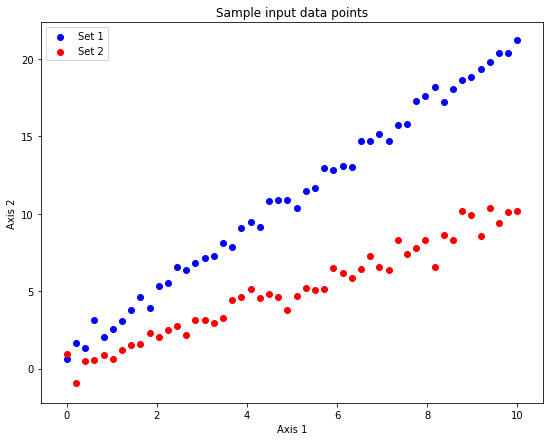
\includegraphics[width=0.3\textheight]{illustrate_p5.png}
	\caption{If the data looks somewhat like this, using multiple mixture of linear regressions would be a better idea.}
	\label{illus}
\end{figure} 

\subsection{Part 2: ALT-OPT Algorithm}

\subsubsection{Estimating the latent variables fixing the parameters}
Suppose we have the optimal value of $\Theta = \hat{\Theta}$, then we can estimate $z_n$ as follows:
\begin{eqnarray}
\hat{z_n} = \arg \max_{k}p(z_n=k| y_n, \textbf{x}_n, \hat{\Theta}) =  \arg \max_{k} \frac{p(y_n, z_n = k| \textbf{x}_n, \hat{\Theta})}{p(y_n|\textbf{x}_n , \hat{\Theta})} \\ 
 =  \arg \max_{k} \frac{p(y_n| z_n = k, \textbf{x}_n , \hat{\Theta})p(z_n = k| \hat{\Theta})}{\sum_{l=1}^{K}p(y_n| z_n = l, \textbf{x}_n , \hat{\Theta})p(z_n = l| \hat{\Theta})} \\
 =  \arg \max_{k} \frac{\pi_k \mathcal{N}(\textbf{w}^{T}_{k}\textbf{x}_n , \beta^{-1})}{\sum_{l=1}^{K}\pi_l \mathcal{N}(\textbf{w}^{T}_{l}\textbf{x}_n , \beta^{-1})}
 \label{eq6}
\end{eqnarray}
Let us denote the term in equation \ref{eq6} as $\gamma_{nk}$. Notice that the denominator does not depend on $k$ and can be dropped, but I am keeping it since the expression takes form of probability. It will not matter for the maximization. Also, let's use the notation that $z_{nk} = 1 \ \textit{iff} \ z_n = k$.

\subsubsection{Estimating the parameters fixing the latent variables}
Once we pick $\hat{z}_n$'s that maximize $\gamma_{nk}$'s, we can now keep them fixed and estimate parameters.
\[
\hat{\Theta} = \arg\max_{\Theta}\mathcal{L}(\Theta, \{\hat{z}_n\}) =  \arg\max_{\Theta} \sum_{n=1}^{N}\log p(y_n, \hat{z}_n | \textbf{x}_n, \Theta)
\]
\[
\hat{\Theta} = \arg\max_{\Theta} \sum_{n=1}^{N}\sum_{k=1}^{K}\hat{z}_{nk}\left[ \log\pi_{k} + \log \mathcal{N}(\textbf{w}^{T}_{k}\textbf{x}_n, \beta^{-1}) \right]
\]
Note that we will also have to incorporate the constraint $\sum_{k}\pi_k = 1$. We can then solve by constrained optimization. For $\pi_k$, since the term involving it is not coupled with any of the other paramters, we can solve for it independently. The problem for finding $\pi_k$ is exactly the same as that in generative classification with known labels (Ref: Lecture 15, Slide 9), so I will use that result directly.
\[
\boxed{\hat{\pi}_k = \frac{1}{N}\sum_{n=1}^{N}\hat{z}_{nk} = \frac{N_k}{N}}
\]
Now, to estimate the weights $\textbf{w}_k$'s, we have
\[
\{\hat{\textbf{w}}_k\}_{k=1}^{K} = \arg\max_{\textbf{w}_1,..,\textbf{w}_K}\sum_{n=1}^{N}\sum_{k=1}^{K}\hat{z}_{nk}(\textbf{w}^{T}_{k}\textbf{x}_n - y_n)^{2}
\]
\[
\{\hat{\textbf{w}}_k\}_{k=1}^{K} = \arg\max_{\textbf{w}_1,..,\textbf{w}_K} \sum_{k=1}^{K}(\textbf{y} - \textbf{X}\textbf{w}_k)^{T}Z_{k}(\textbf{y} - \textbf{X}\textbf{w}_k) \text{ where } Z_{k} = \text{Diag}(z_{1k},..,z_{Nk})
\]
Note that these terms can be maximized independently since they do not depend upon each other. Thus, we get
\[
\hat{\textbf{w}}_k = \arg \max_{\textbf{w}_k}(\textbf{y} - \textbf{X}\textbf{w}_k)^{T}Z_{k}(\textbf{y} - \textbf{X}\textbf{w}_k)
\]
This is the same as solving a linear regression problem with examples being weighted by $\{z_{nk}\}$'s. Thus, the solution (Ref: Practice Problem Set 1, Q.5) will be as follows:
\[
\boxed{\hat{\textbf{w}}_k = [\textbf{X}^{T}Z_{k}\textbf{X}]\textbf{X}^{T}Z_{k}\textbf{y}}
\]

\subsubsection{A Special case}
For the case when $\pi_k = (1/K), \ \forall k = 1,2,..K$ implies that 
\[
\hat{z}_n = \arg\max_{k} \delta_{nk} = \arg\max_{k} \frac{ \mathcal{N}(\textbf{w}^{T}_{k}\textbf{x}_n , \beta^{-1})}{\sum_{l=1}^{K} \mathcal{N}(\textbf{w}^{T}_{l}\textbf{x}_n , \beta^{-1})}
\]
This kind of an update ignores the number of points that can be explained by a single model $\textbf{w}_k$. Thus, it will only consider the probability of $x_n$ explained by these different models giving them equal weightage.

\subsection{Part 3A: EM Algorithm}

\subsubsection{A. Computing the posterior}

We have already computed the conditional distribution for the latent variables in equation \ref{eq6}. 
\[
\boxed{p(z_n = k| y_n, \textbf{x}_n, \Theta) = \gamma_{nk} = \frac{\pi_k \mathcal{N}(\textbf{w}^{T}_{k}\textbf{x}_n , \beta^{-1})}{\sum_{l=1}^{K}\pi_l \mathcal{N}(\textbf{w}^{T}_{l}\textbf{x}_n , \beta^{-1})}}
\]
From the discrete distribution, we have the expectation as simply:
\[
\mathbb{E}[z_n] = \sum_{k=1}^{K}kp(z_n = k| y_n, \textbf{x}_n, \Theta) = \sum_{k=1}^{K}k\gamma_{nk}
\]
\begin{equation}
\label{eq7}
\mathbb{E}[z_{nk}] = 1*p(z_{nk} = 1) + 0*p(z_{nk}=0) = p(z_{n} = k) = \gamma_{nk} 
\end{equation}

\subsubsection{B. Computing the expected CLL}
Now, let us compute the expected CLL.
\[
CLL = \log p(Y, Z| X, \Theta) = \sum_{n=1}^{N}\log p(y_n, z_n|\textbf{x}_n, \Theta) =  \sum_{n=1}^{N}\sum_{k=1}^{K}z_{nk}\left[ \log\pi_{k} + \log \mathcal{N}(\textbf{w}^{T}_{k}\textbf{x}_n, \beta^{-1}) \right]
\]
\begin{equation}
\mathbb{E}[CLL] = \sum_{n=1}^{N}\sum_{k=1}^{K}\mathbb{E}[z_{nk}]\left[ \log\pi_{k} + \log \mathcal{N}(\textbf{w}^{T}_{k}\textbf{x}_n, \beta^{-1}) \right]
\label{eq8}
\end{equation}
We can get $\mathbb{E}[z_{nk}]$ from equation \ref{eq7}, and thus the expected CLL. The rest of the procedure for maximizing the expected CLL will remain the same as in previous part except that instead of $z_{nk}$, we will be using $\gamma_{nk}$. Thus, we have

\begin{equation}
\boxed{\hat{\pi}_k = \frac{1}{N}\sum_{n=1}^{N}\gamma_{nk}}
\label{eq9}
\end{equation}

\begin{equation}
\boxed{\hat{\textbf{w}}_k = [\textbf{X}^{T}\Gamma_{k}\textbf{X}]\textbf{X}^{T}\Gamma_{k}\textbf{y}}
\label{eq10}
\end{equation}
where $\Gamma_{k} = \text{Diag}(\gamma_{1k}, \gamma_{2k},.., \gamma_{nk})$.

\subsubsection{C. The Algorithm}
\begin{enumerate}
	\item Initialize $\Theta = \Theta^{(0)} = \{\pi^{(0)}_{k}, \textbf{w}^{(0)}_k\}$, set $t = 1$
	\item \textbf{E step}: Now, assuming the values of $\Theta^{(t-1)}$, compute the expected CLL from equation \ref{eq8} using expression for $\mathbb{E}[z_{nk}] = \gamma_{nk}$.
	\item \textbf{M step}: Now, update the values for $\pi^{(t)}_{k}, \textbf{w}_{k}^{(t)}$ using the equations \ref{eq9}, \ref{eq10}. Update $t = t+1$.
	\item Repeat steps 2-4 until convergence.
\end{enumerate}

\section{Part 3B: Particular case}
We have to show that when $\beta\rightarrow \infty$, the EM algorithm boils down to the ALT-OPT algorithm. Basically, we want to show the following:
\[
\gamma_{nk} = 1 \ \textit{iff} \ k_{*} = \arg\max_{k}\frac{\pi_k \mathcal{N}(\textbf{w}^{T}_{k}\textbf{x}_n , \beta^{-1})}{\sum_{l=1}^{K}\pi_l \mathcal{N}(\textbf{w}^{T}_{l}\textbf{x}_n , \beta^{-1})}
\]
We have 
\[
\gamma_{nk}(\beta)  =   \frac{\pi_{k}\exp\left[ -\beta^{2} \Vert y_n - \textbf{w}^{T}_{k}\textbf{x}_{n} \Vert^{2} \right]}{\sum_{l=1}^{K}\pi_{l}\exp\left[ -\beta^{2} \Vert y_n - \textbf{w}^{T}_{l}\textbf{x}_{n} \Vert^{2} \right]}
\]
\[
\Rightarrow \gamma_{nk}(\beta)  = \frac{1}{1 + \sum_{l\neq k} \frac{\pi_{l}}{\pi_{k}}\exp\left[ -\beta^{2} (\Vert y_n - \textbf{w}^{T}_{l}\textbf{x}_{n} \Vert^{2} - \Vert y_n - \textbf{w}^{T}_{k}\textbf{x}_{n} \Vert^{2}) \right]}
\]
Now, consider the case when $k \neq  k_{*}$ as defined above, the term $\Vert y_n - \textbf{w}^{T}_{l}\textbf{x}_{n} \Vert^{2} - \Vert y_n - \textbf{w}^{T}_{k}\textbf{x}_{n} \Vert^{2} < 0 , \forall l = k_{*}$, thus the exponent becomes $\infty$ making $\gamma_{nk}\rightarrow 0$. For $k = k_{*}$, clearly, all other terms will go to $0$, and thus $\gamma_{nk_{*}} = 1$. Thus, the claim is proved and hence we will have
\[
\mathbb{E}[z_{nk}] = 1 \text{ only when } \hat{z}_{nk} = 1
\]
This implies that the expectation step becomes the same as that of ALT-OPT and so does maximization since the expected likelihood will be the same that the paramtere update step in ALT-OPT.
\end{mlsolution}

\begin{mlsolution}
\section{Programming Problem 1}
\subsection{1. Kernel Ridge Regression}
\textbf{Observations}: In Kernel ridge regression, an important observation was that the mean squared error increases on increasing $\lambda$. This is expected since lower $\lambda$ implies overfitting while increasing $\lambda$ means too simple model and thus underfits. Refer to figures \ref{1a}, \ref{1b}, \ref{1c} and \ref{1d} for plots and table \ref{tab-1a} for mean squared error.
\begin{figure}[!htbp]
	\label{fig1a}
	\begin{subfigure}{0.5\textwidth}
		\centering
		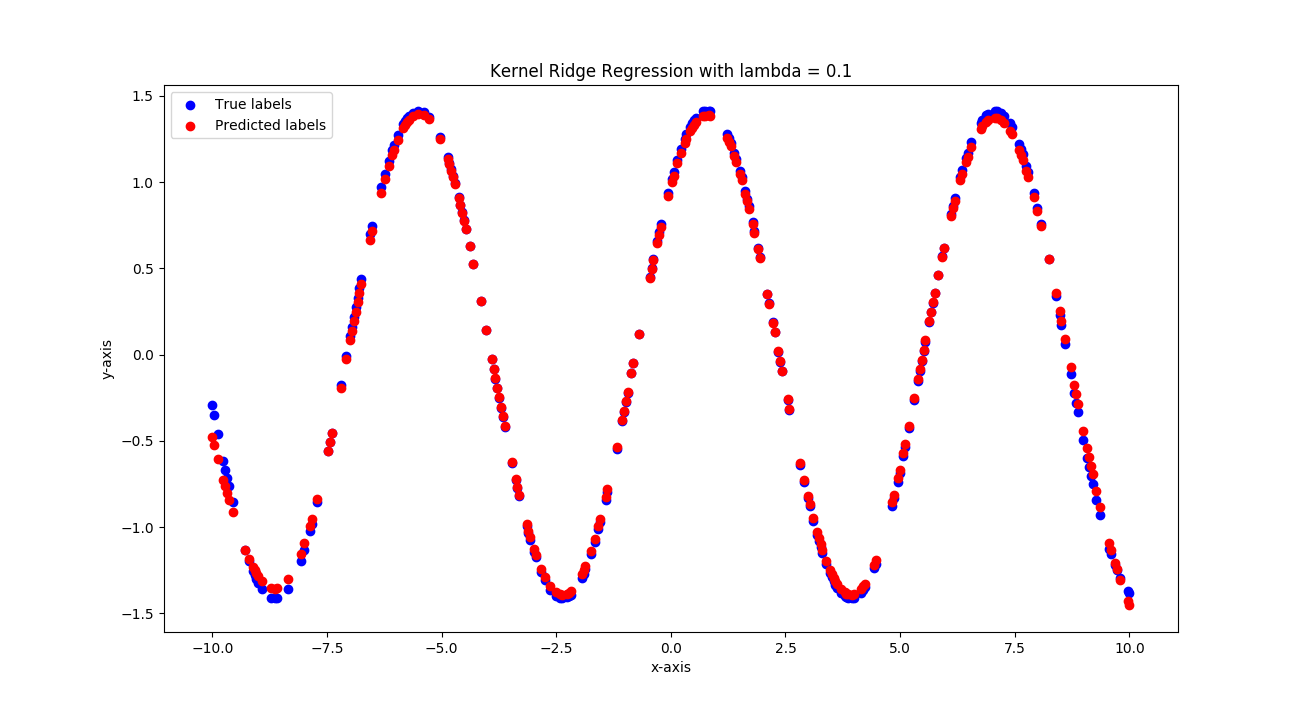
\includegraphics[width=1.8\textwidth]{images/krr_0.png}
		\caption{1a}
		\label{1a}
	\end{subfigure}
\\
	\begin{subfigure}{0.5\textwidth}
		\centering
		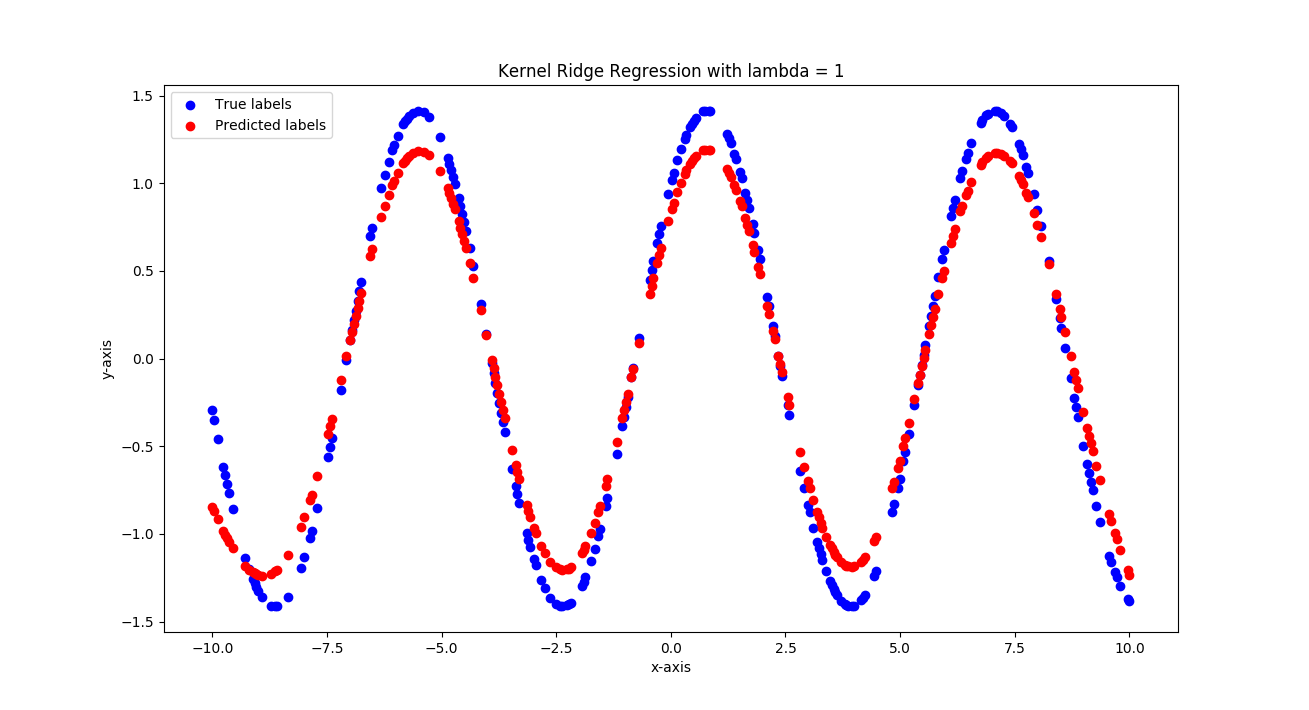
\includegraphics[width=1.8\textwidth]{images/krr_1.png}
		\caption{1b}
		\label{1b}
	\end{subfigure}
\end{figure}

\begin{figure}[!htbp]
	\label{fig1b}
	\begin{subfigure}{0.5\textwidth}
		\centering
		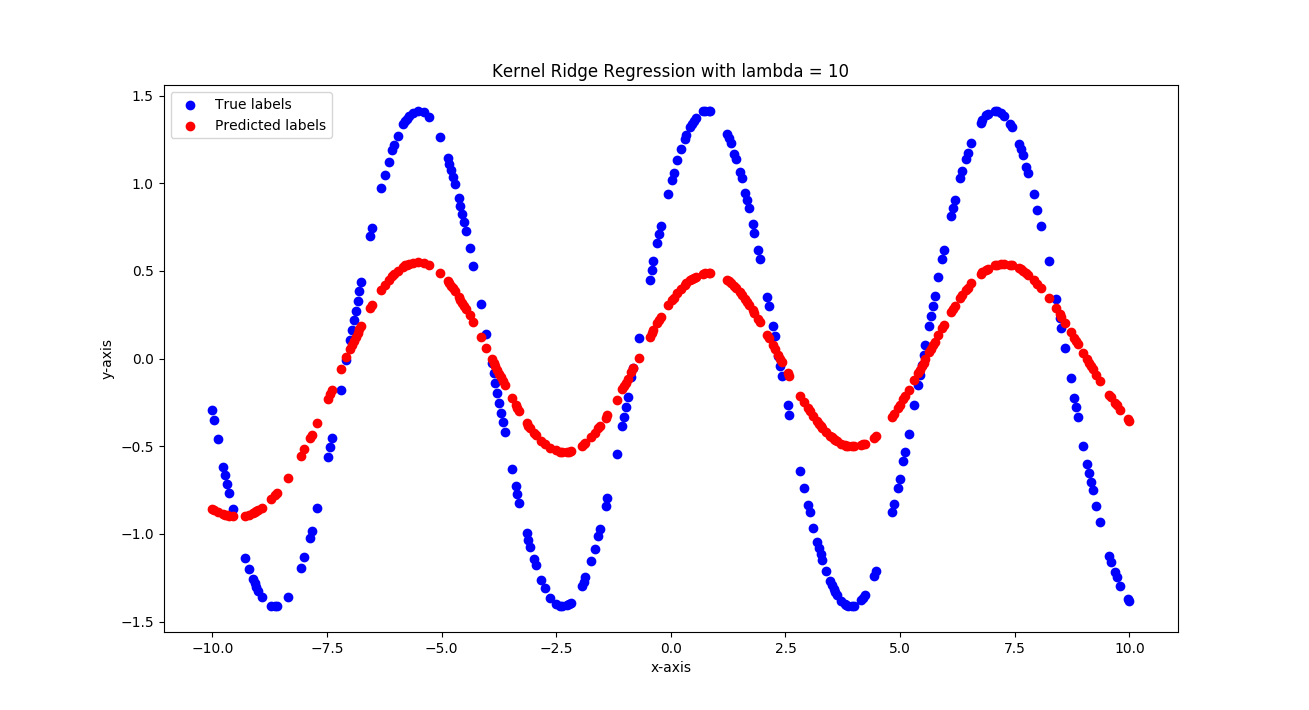
\includegraphics[width=1.8\textwidth]{images/krr_10.png}
		\caption{1c}
		\label{1c}
	\end{subfigure}
	\\
	\begin{subfigure}{0.5\textwidth}
		\centering
		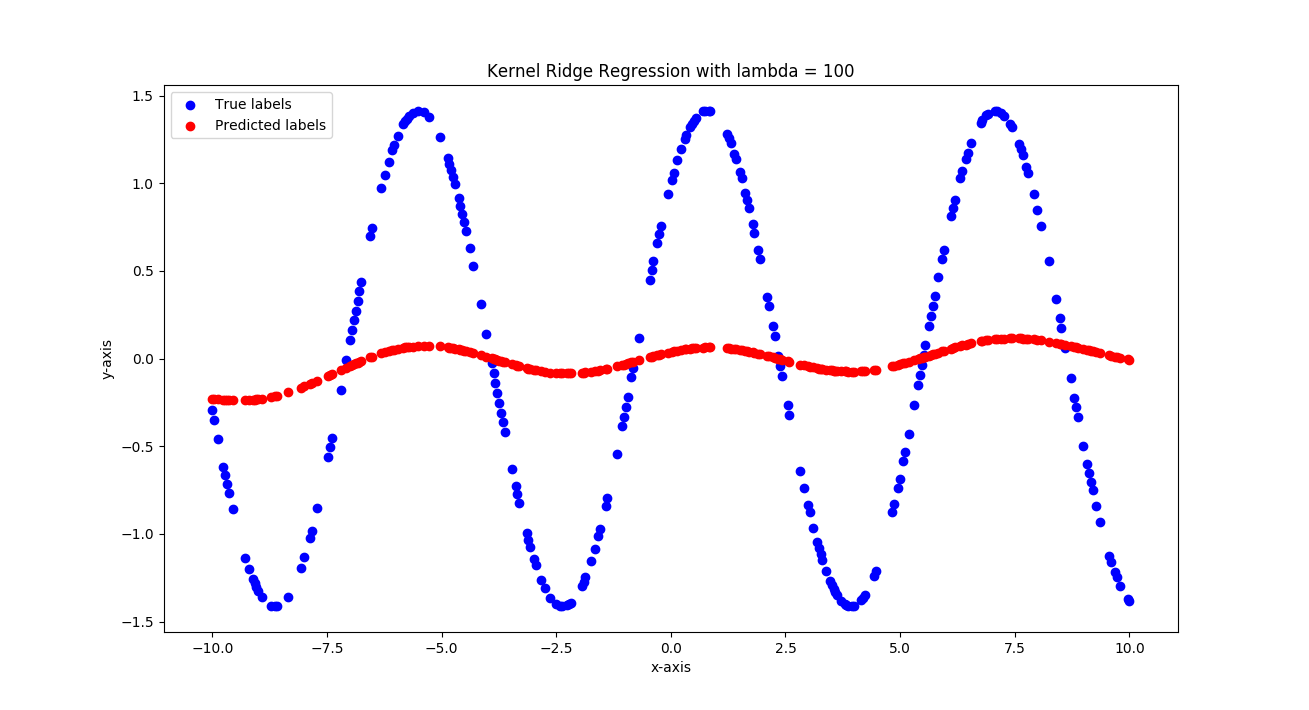
\includegraphics[width=1.8\textwidth]{images/krr_100.png}
		\caption{1d}
		\label{1d}
	\end{subfigure}
\end{figure}

\begin{table}[!htbp]
	
	\begin{center}
		\begin{tabular}{|c|c|c|}
			
			\hline
			\hspace{4mm}$\lambda$\hspace{4mm} & \hspace{4mm}\textbf{Mean Squared Error}\hspace{4mm} \\
			\hline
			\hline
			0.1 & 0.00107 \\
			\hline
			1 & 0.02944 \\ 
			\hline
			10 & 0.37461 \\
			\hline
			100 & 0.83259 \\
			\hline
		\end{tabular}
	\end{center}
	\label{tab-1a}
	\caption[MSE for Kernel-ridge]{As we increase the regularization hyperparameter $\lambda$, the mean squared error increases. Clearly, as evident from the plots as well, $\lambda = 0.1$ coressponds to overfit model whereas $\lambda = 100$ corressponds to an underfit model. The model with $\lambda = 1$ seems to be appropriate.}
\end{table}

\subsection{2. Landmark-ridge Regression}

\textbf{Observations}: The key observation is that the mean squared error decreases as we increase $L$ upto a point and then remains more or less the same  (look at the change from $L = 50$ to $L = 100$). Using too low value of $L$ means that the model is based upon information of a very few data points and these datapoints may not capture all the characteristics of the global dataset. For an extremely high value of $L$, it will be almost similar to using all the points in the dataset, also, it is important to notice that increasing $L$ implies higher cost of computations since the dimension of feature space increases. Refer to figures \ref{2a}, \ref{2b}, \ref{2c}, \ref{2d} and \ref{2e} for plots and table \ref{tab-2a} for mean squared error.
\begin{figure}[!htbp]
	\begin{subfigure}{0.5\textwidth}
		\centering
		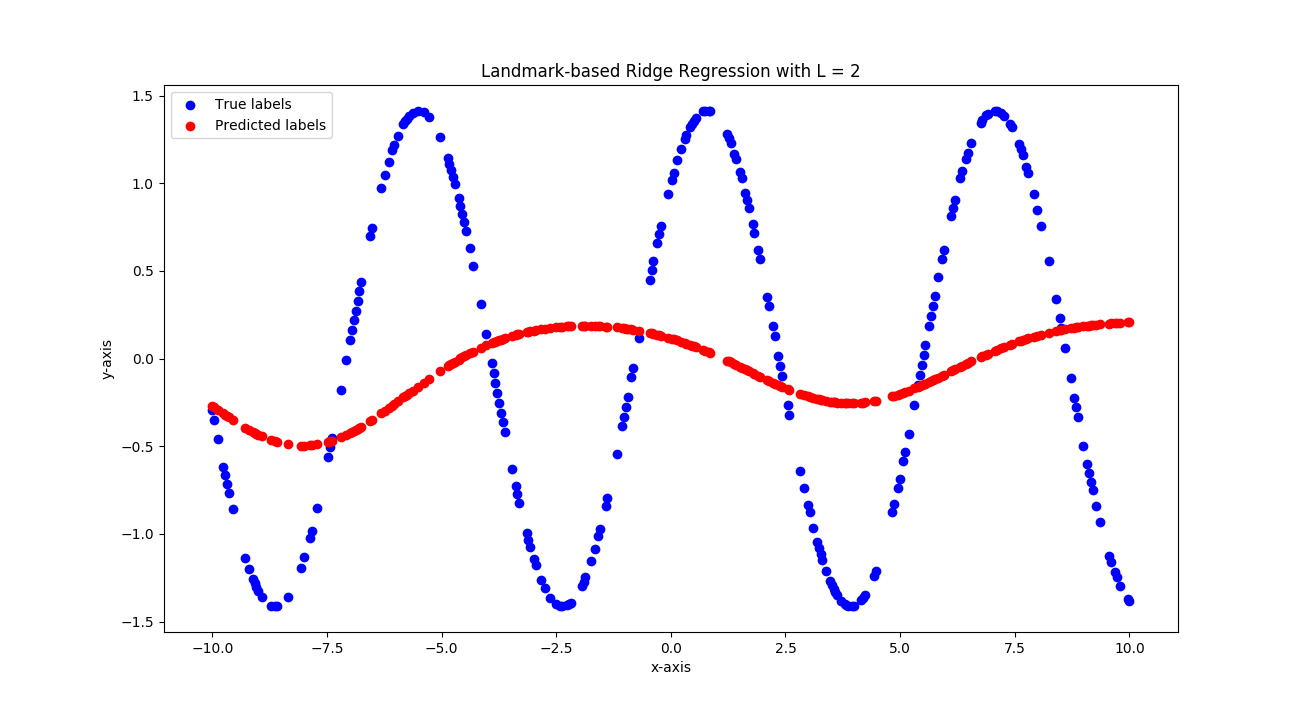
\includegraphics[width=1.8\textwidth]{images/lrr_L2.png}
		\caption{1a}
		\label{2a}
	\end{subfigure}
	\\
	\begin{subfigure}{0.5\textwidth}
		\centering
		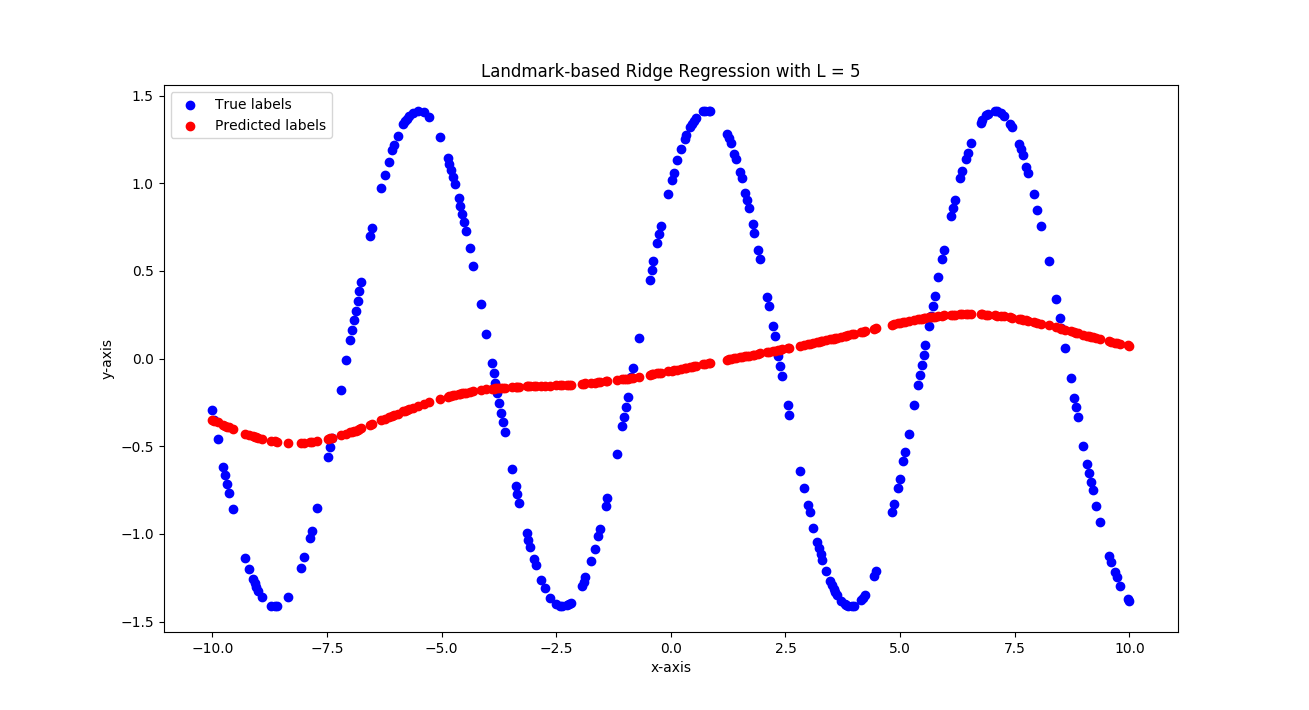
\includegraphics[width=1.8\textwidth]{images/lrr_L5.png}
		\caption{1b}
		\label{2b}
	\end{subfigure}
\end{figure}

\begin{figure}[!htbp]
	\begin{subfigure}{0.5\textwidth}
		\centering
		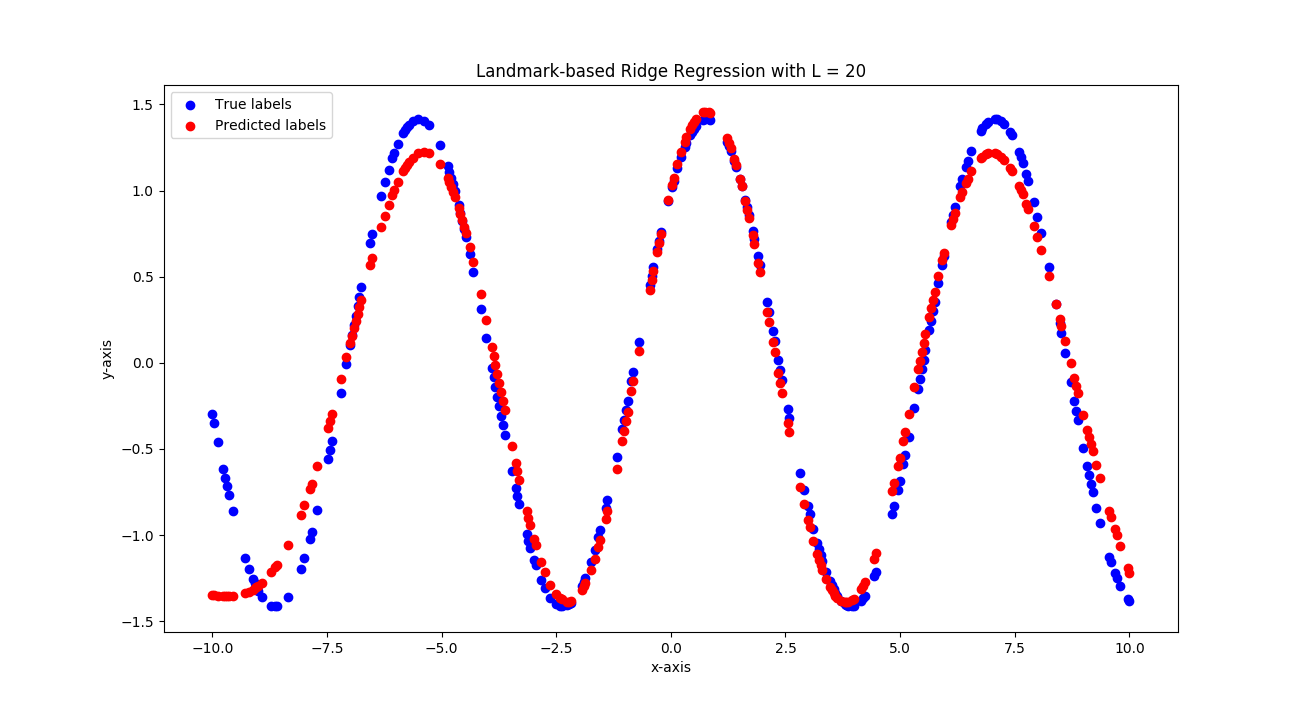
\includegraphics[width=1.8\textwidth]{images/lrr_L20.png}
		\caption{1c}
		\label{2c}
	\end{subfigure}
	\\
	\begin{subfigure}{0.5\textwidth}
		\centering
		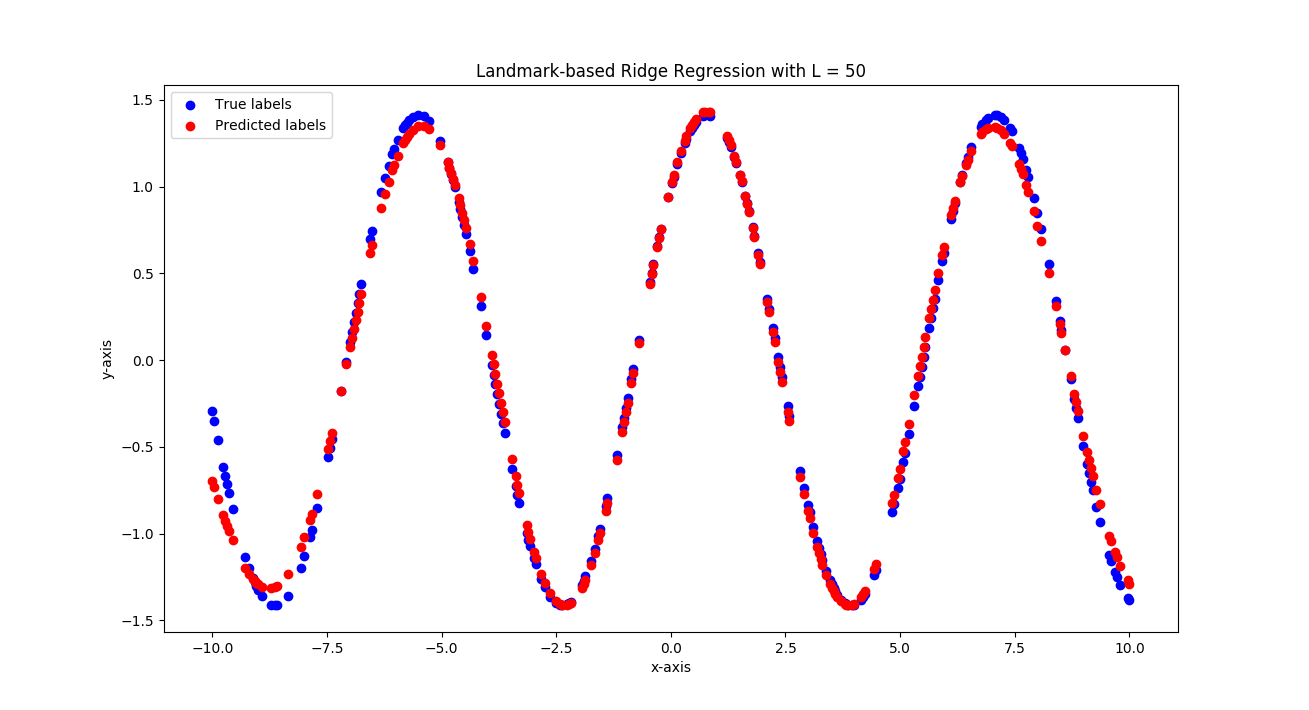
\includegraphics[width=1.8\textwidth]{images/lrr_L50.png}
		\caption{1d}
		\label{2d}
	\end{subfigure}
\\
	\begin{subfigure}{0.5\textwidth}
		\centering
		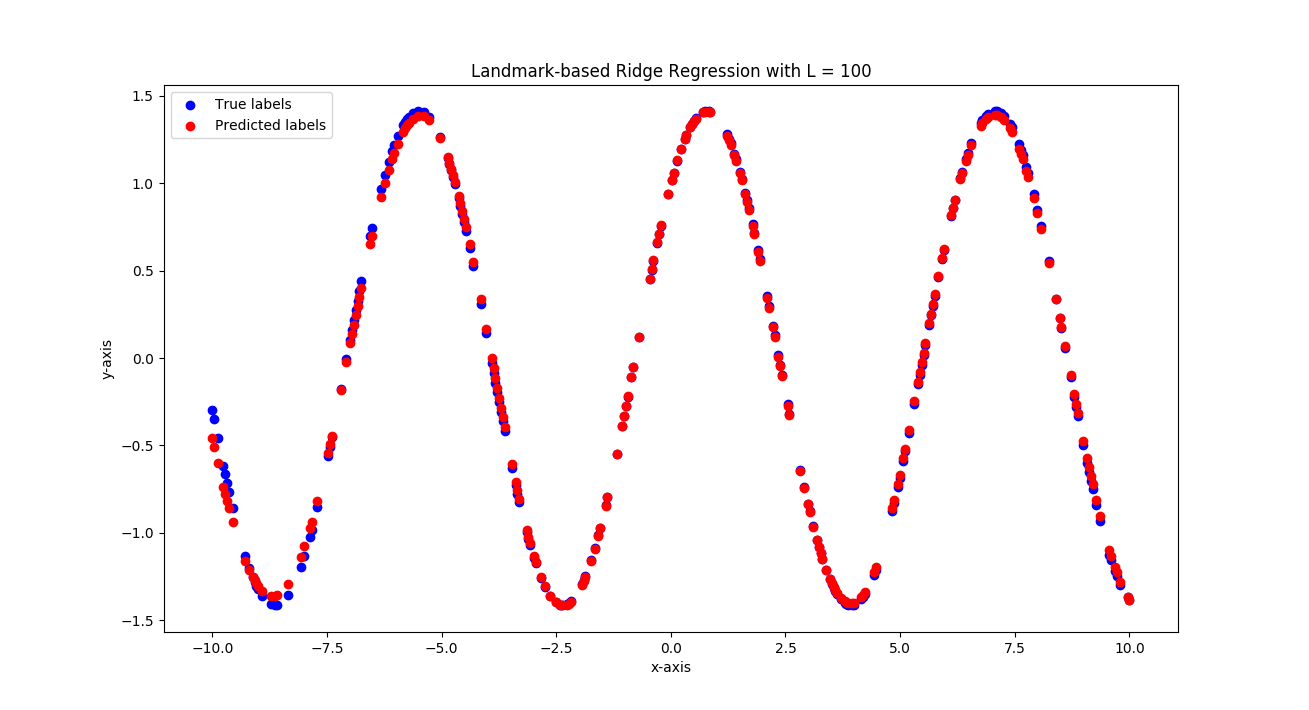
\includegraphics[width=1.8\textwidth]{images/lrr_L100.png}
		\caption{2e}
		\label{2e}
	\end{subfigure}
\end{figure}

\begin{table}[!htbp]
	\label{tab-2a}
	\begin{center}
		\begin{tabular}{|c|c|c|}
			\hline
			\hspace{4mm}$L$\hspace{4mm} & \hspace{4mm}\textbf{Mean Squared Error}\hspace{4mm} \\
			\hline
			\hline
			2 & 0.95181 \\
			\hline
			5 & 0.39178 \\ 
			\hline
			20 & 0.00905 \\
			\hline
			50 & 0.00142 \\
			\hline
			100 & 0.00182 \\
			\hline
		\end{tabular}
	\end{center}
	\caption[MSE for Landmark-ridge]{As we increase the value of $L$, the mean squared error decreases. Clearly, as evident from the plots as well, $L = 100$ coressponds to perfectly fit model whereas $L = 1$ corressponds to an excessively underfit model. The model with $L = 50$ seems to be a pretty good approximation.}
\end{table}


\section{Programming Problem 2}
\subsection{1. Using Hand-crafted Features}
I have used the following three-dimensional feature transformation for clustering:
\[
f: \mathbb{R}^{2} \rightarrow \mathbb{R}^{3} \Rightarrow f(x_1, x_2) = (x_1, x_2, x^{2}_{1}+x^{2}_{2})
\]
I wanted a feature transformation that will split the dataset into two clusters and that the two transformed clusters will be smooth and seperated. From the data visualization, it seemed that the invariant binding each of the clusters was the inner and outer radius os the two concentric clusters. Refer to figure \ref{t-space} for visual results.

\begin{figure}[!htbp]
	
	\begin{subfigure}{0.5\textwidth}
		\centering
		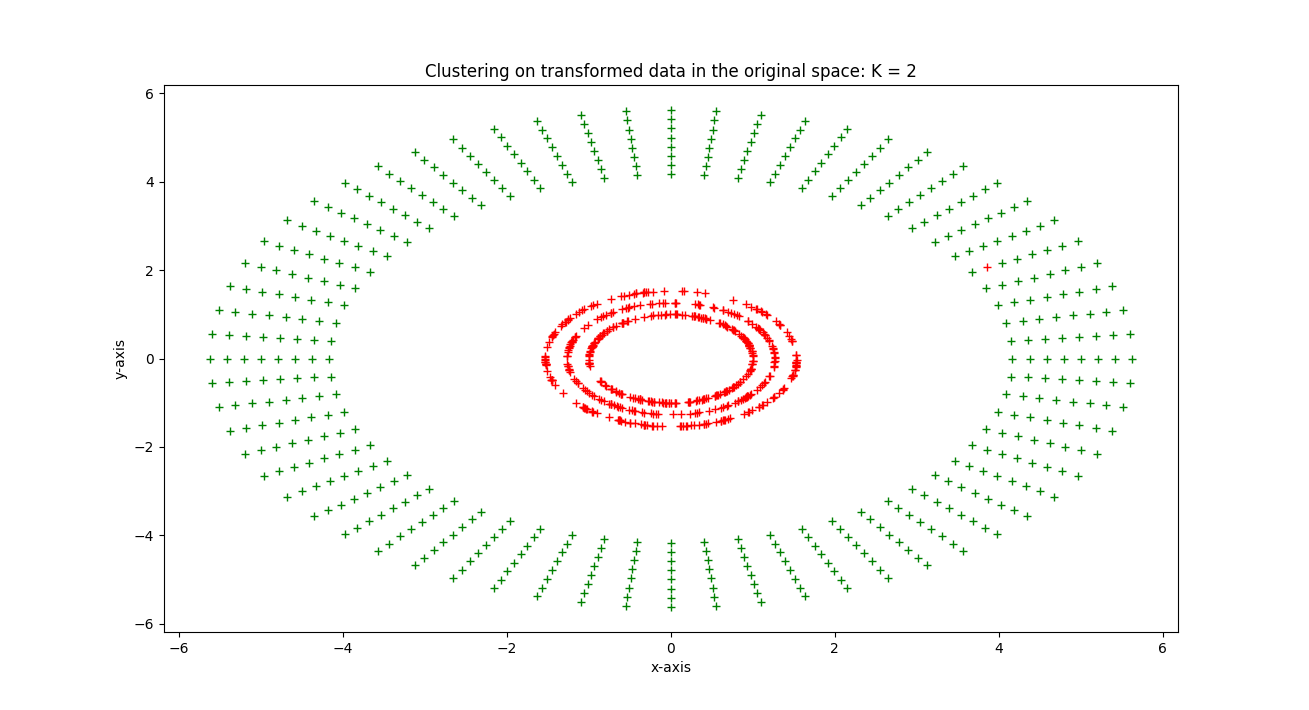
\includegraphics[width=1.8\textwidth]{images/original_space.png}
		\caption{Dataset in original space with clusters}
		\label{t-space}
	\end{subfigure}

\end{figure}


\subsection{2. Using Kernels}
Using landmark based approach with RBF kernels, I observed that the clustering is very sensitive to the choice of landmark ($L=1$) point. The clustering is such that one of the clusters is centered around the landmark point and the rest is the second cluster. A good cluster may be obtained if the randomly chosen landmark point lands into the innermost part of the inner cluster. Note that this is expected since clustering assumes equal spread of clusters and spherical clusters. thus if the landmark point lies in inner cluster, one of the clusters centers around it (since, the new feature space is based on distance from the landmark) and the rest becomes the other cluster.
Refer to following figures  for results.
\begin{figure}[!htbp]
	\begin{subfigure}{0.5\textwidth}
		\centering
		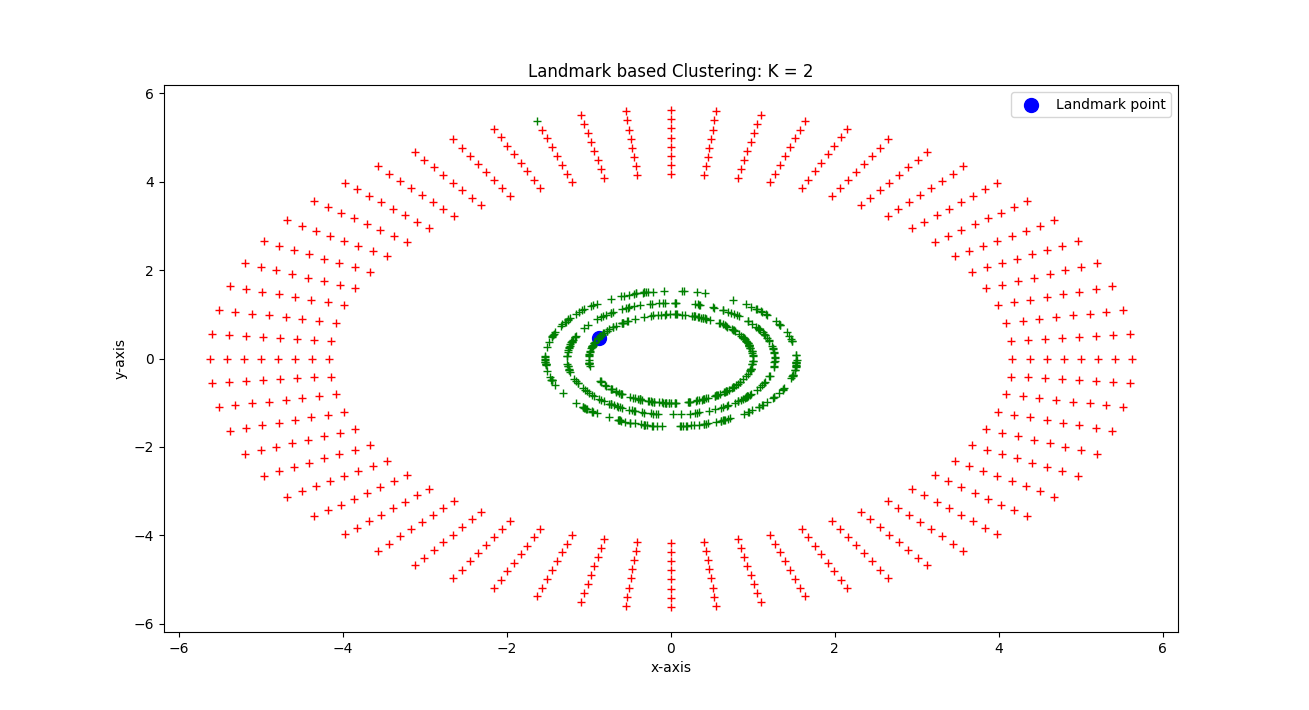
\includegraphics[width=1.1\textwidth]{images/l_random1.png}
		\caption{}
		\label{l1}
	\end{subfigure}
	\begin{subfigure}{0.5\textwidth}
		\centering
		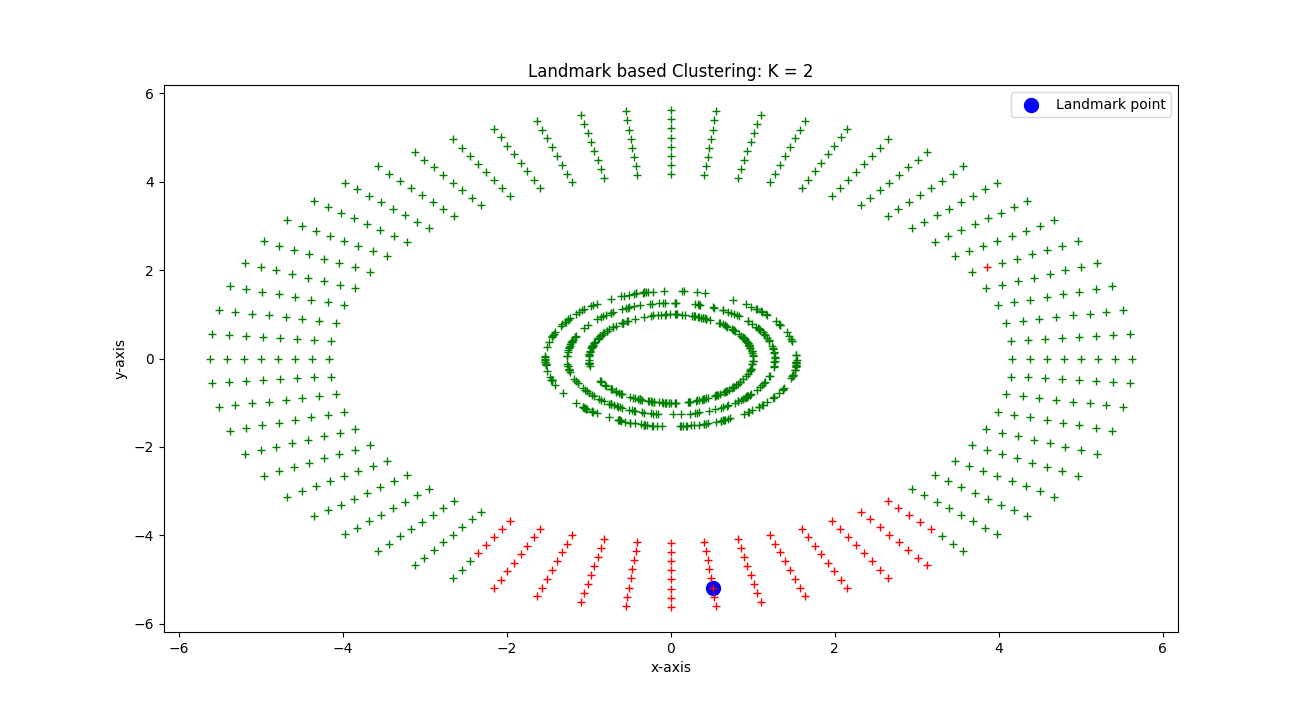
\includegraphics[width=1.1\textwidth]{images/l_random2.png}
		\caption{}
		\label{l2}
	\end{subfigure}
\\
	\begin{subfigure}{0.5\textwidth}
		\centering
		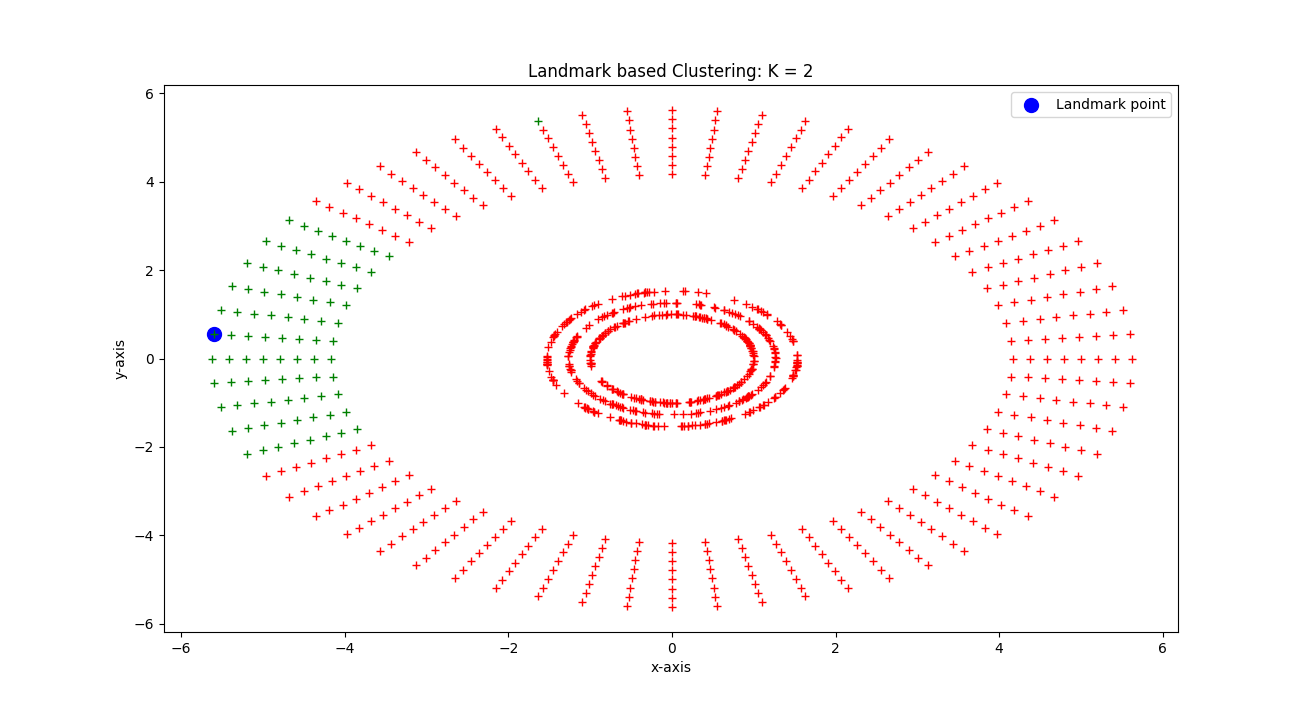
\includegraphics[width=1.1\textwidth]{images/l_random3.png}
		\caption{}
		\label{l3}
	\end{subfigure}
	\begin{subfigure}{0.5\textwidth}
		\centering
		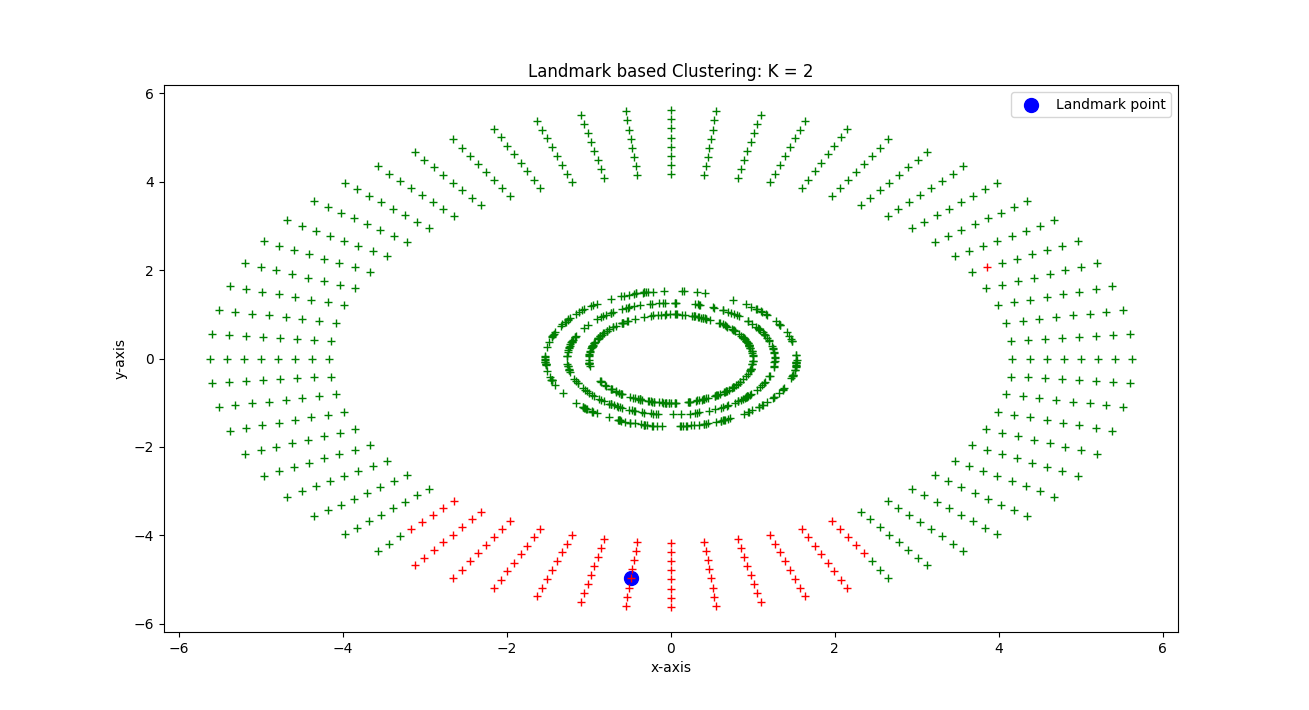
\includegraphics[width=1.1\textwidth]{images/l_random4.png}
		\caption{}
		\label{l4}
	\end{subfigure}
\\
	\begin{subfigure}{0.5\textwidth}
		\centering
		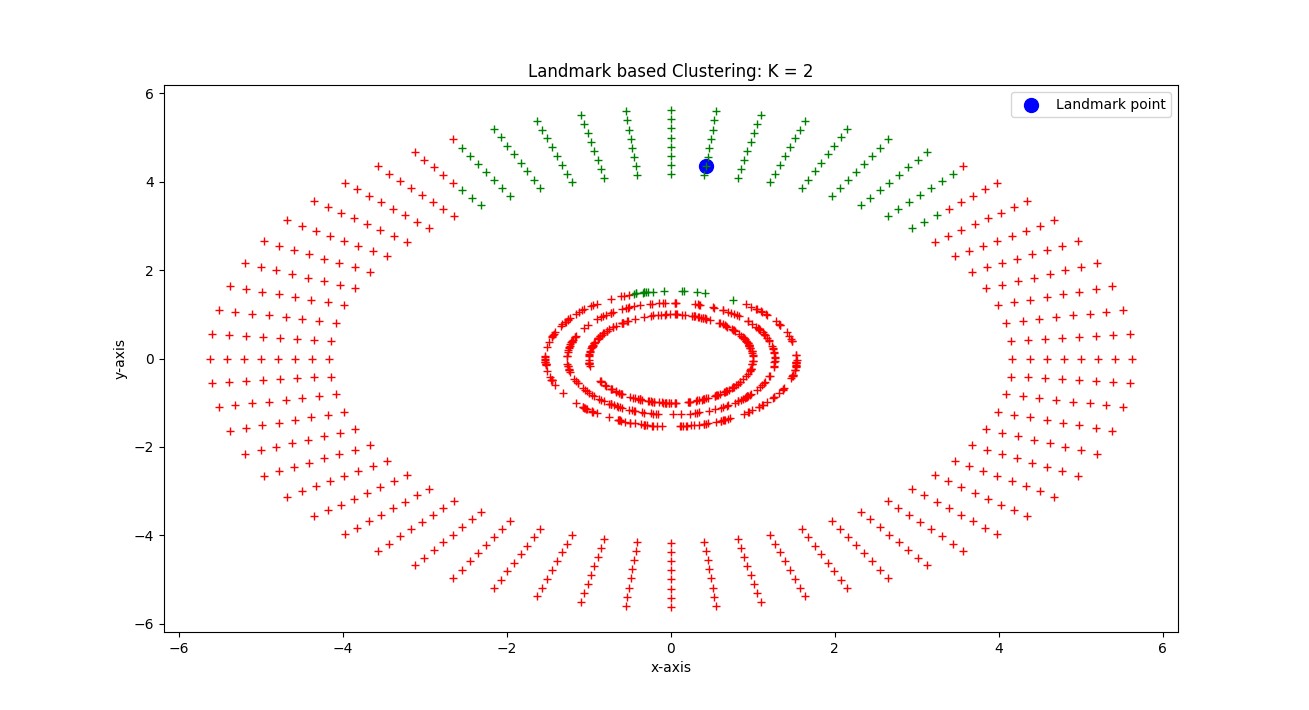
\includegraphics[width=1.1\textwidth]{images/l_random5.png}
		\caption{}
		\label{l5}
	\end{subfigure}
	\begin{subfigure}{0.5\textwidth}
		\centering
		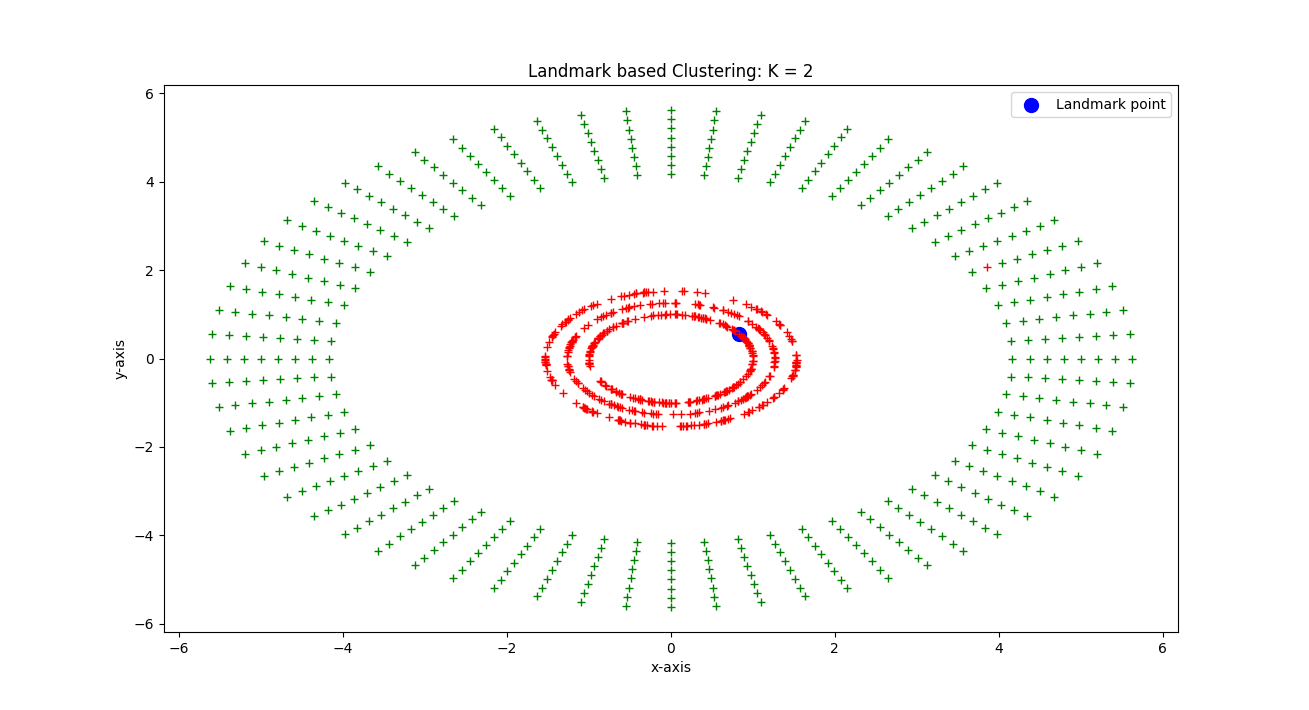
\includegraphics[width=1.1\textwidth]{images/l_random6.png}
		\caption{}
		\label{l6}
	\end{subfigure}
\\
	\begin{subfigure}{0.5\textwidth}
		\centering
		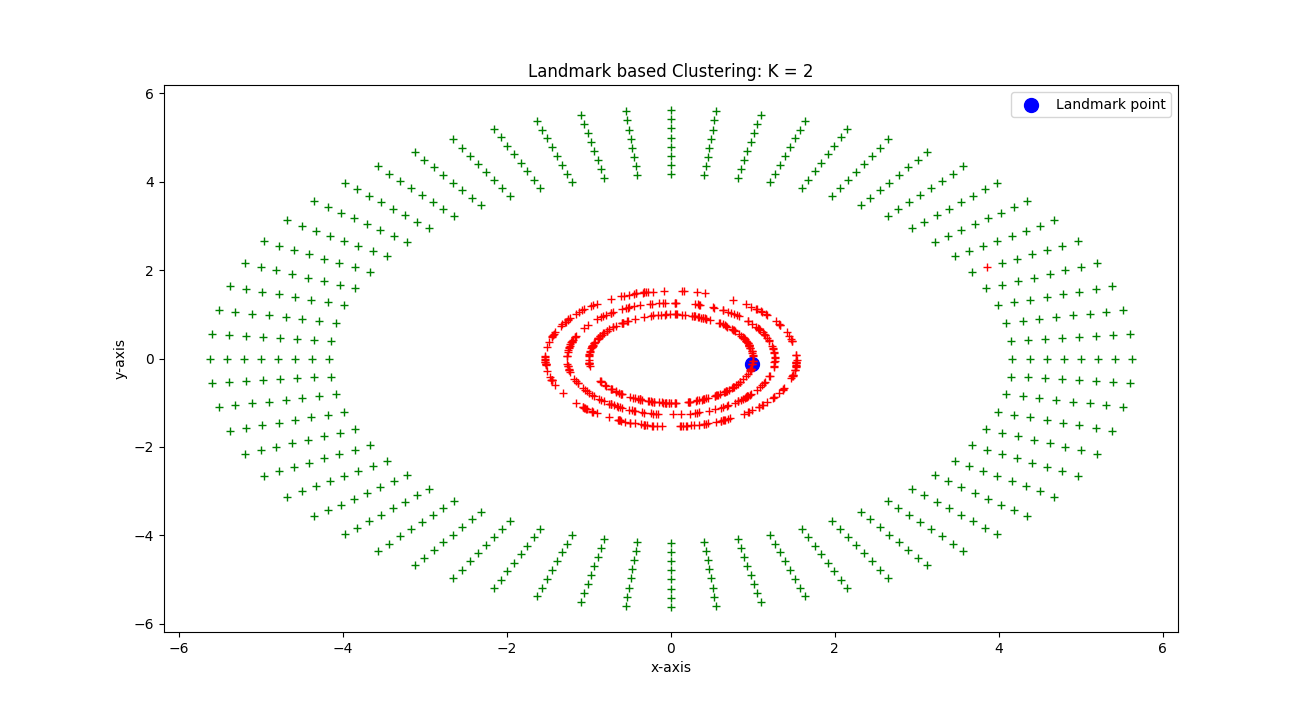
\includegraphics[width=1.1\textwidth]{images/l_random7.png}
		\caption{}
		\label{l7}
	\end{subfigure}
	\begin{subfigure}{0.5\textwidth}
		\centering
		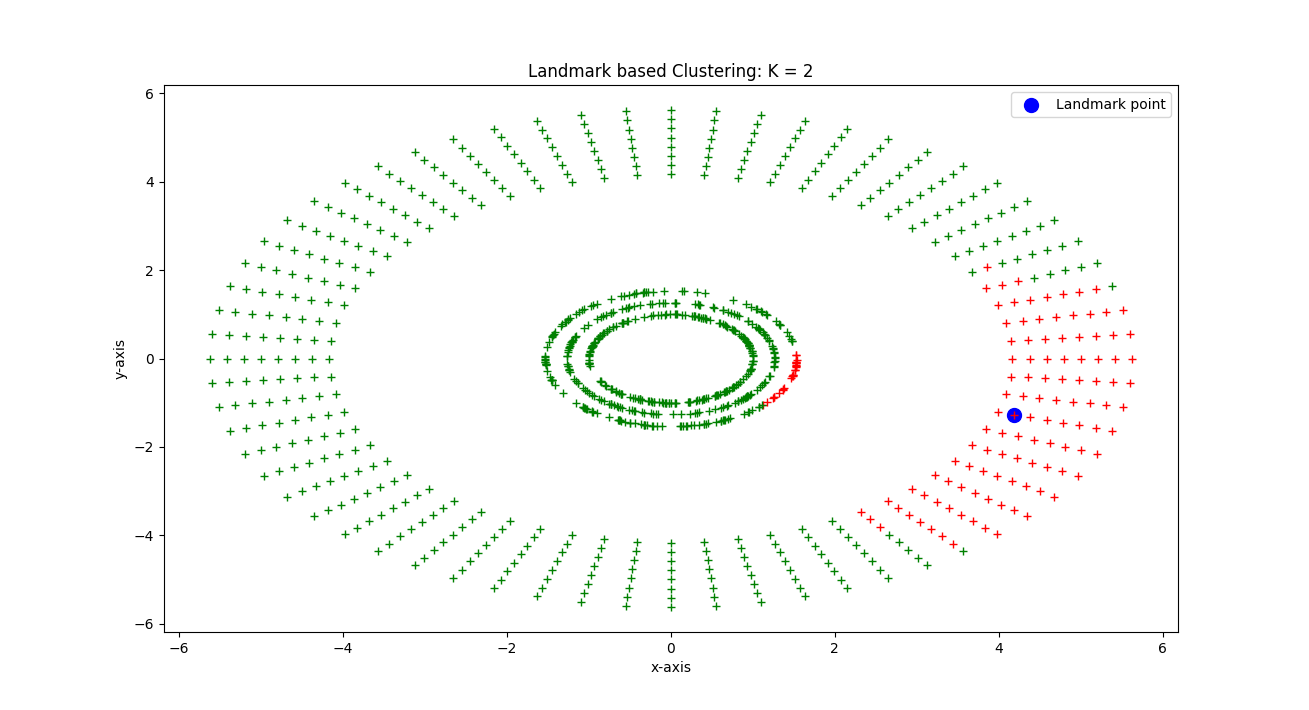
\includegraphics[width=1.1\textwidth]{images/l_random8.png}
		\caption{}
		\label{l8}
	\end{subfigure}
\\
	\begin{subfigure}{0.5\textwidth}
		\centering
		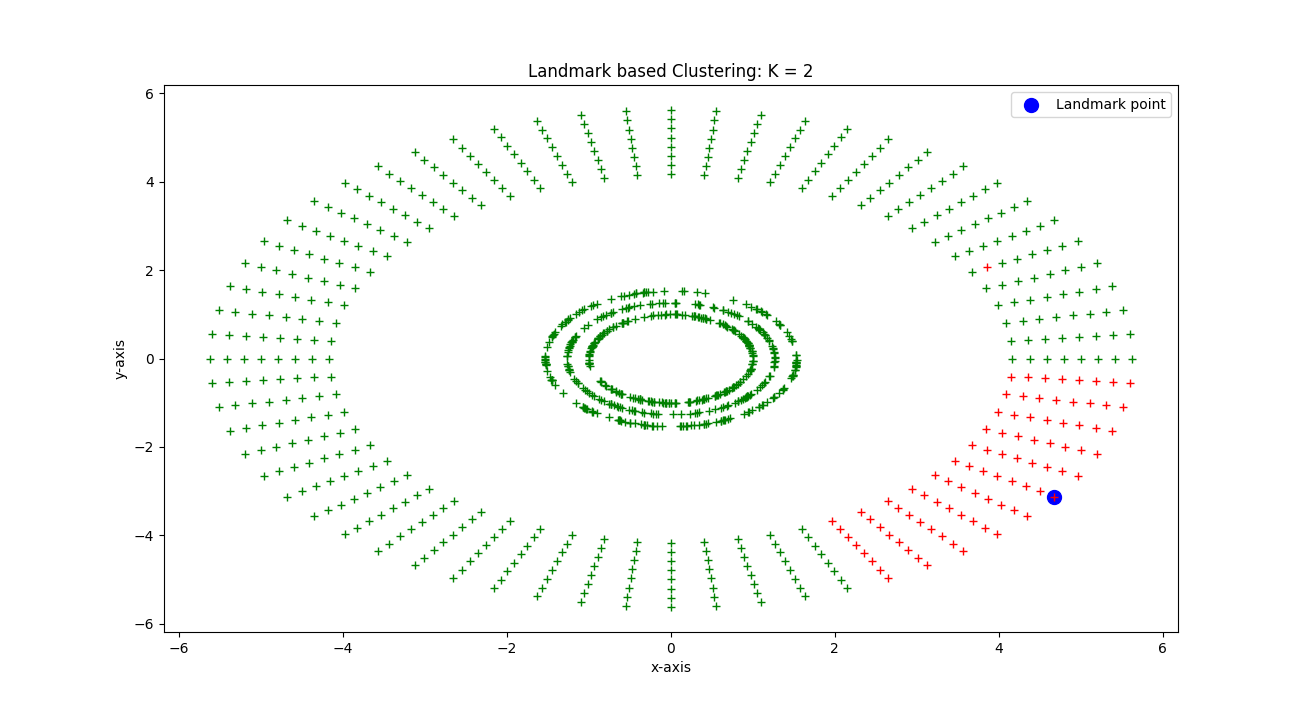
\includegraphics[width=1.1\textwidth]{images/l_random9.png}
		\caption{}
		\label{l9}
	\end{subfigure}
	\begin{subfigure}{0.5\textwidth}
		\centering
		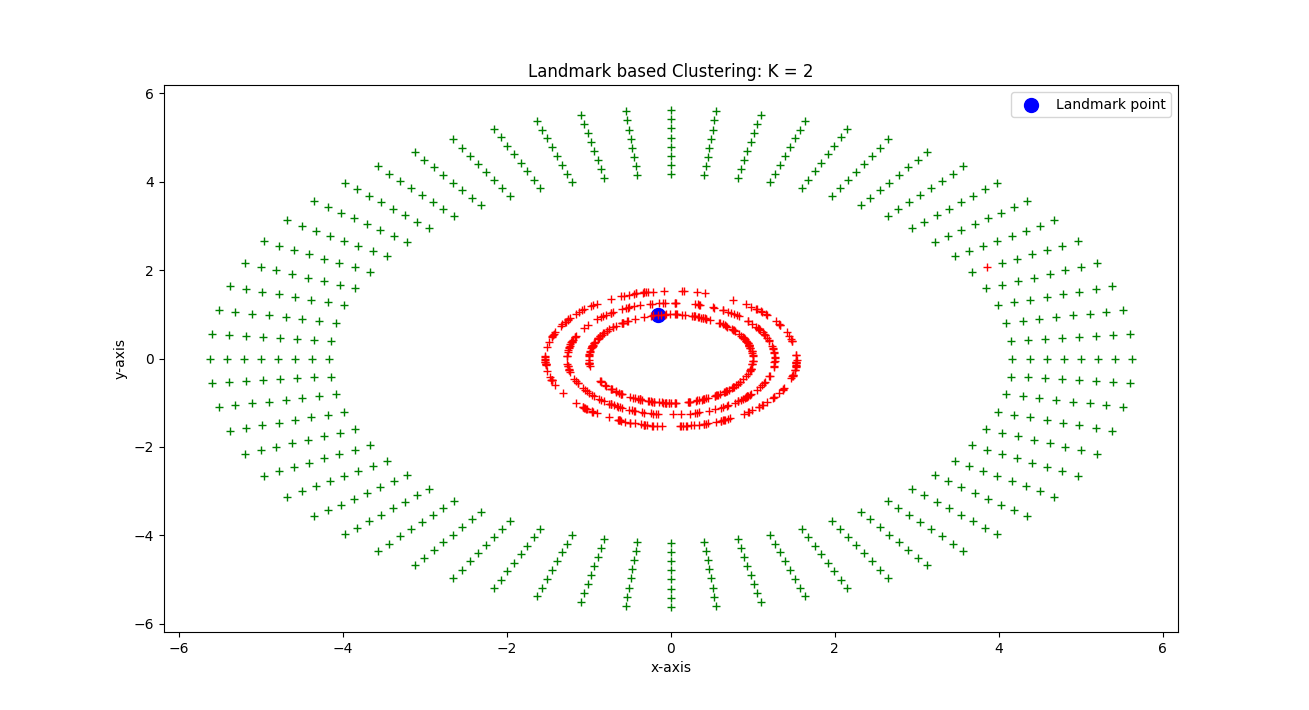
\includegraphics[width=1.1\textwidth]{images/l_random10.png}
		\caption{}
		\label{l10}
	\end{subfigure}
\end{figure}
\end{mlsolution}


\end{document}
